%!TEX root = /Users/zolkko/Projects/zolkko-alarm/doc/main.tex
\section{Реализация программно-аппаратного универсальной
системы терморегулирования на базе микроконтроллера AVR семейства XMega}
В качестве объекта исследования в ходе выполнения дипломного проектирования мной
была спроектирован и частично реализован программно-аппаратный комплекс
универсального терморегулирования.

Одной из возможных областей применения такого рода комплексов является дистанционное
автоматизированное управление коптильными камерами, используемыми при изготовлении
колбасных изделий фабрик пищевой промышленности.

\subsection{Описание структурной схемы универсальной системы терморегулирования}
Структурная схема универсальной системы терморегулирования на базе микроконтроллера
AVR семейства XMega приведена в приложении A.

Функциональным назначением представленных на схеме блоков является:
\begin{enumerate}
	\item{} Управляющее устройство -- устройство устанавливаемое непосредственно
	на объект управления. Выполняет следующие функции:
		\begin{itemize}
			\item{} ОУ -- считывание показаний термопар и усиление их сигнала;
			\item{} устройство индикации -- выводтинформацию о текущем состоянии системы;
			\item{} память -- сранит настройки системы и список технологических процессов для
				исполнения;
			\item{} звуковая сигнализация -- выполняет оповещение звуковым сигналом о
				наступлении события завершения текущей операции или о том, что произошла ошибка;
			\item{} устройство ввода -- обеспечивает функцию задания операции на исполнение,
				остановку операции исполнения;
			\item{} датчик температуры -- получение температур холодного спая термопары;
			\item{} блок ШИМ управления -- формирует управляющий сигнал, воздействующий на
				тепло-электро нагреватель;
			\item{} сетевой интерфейс -- обеспечивает функцию передачи и приёма данных
				через сеть Ethernet 802.3;
			\item{} центральный процессов -- модуль обеспечивающий взаимодействие компонентов
				управляющего устройства, направленное на исполнение заданного технологического
				процесса.
		\end{itemize}
	\item{} Контролирующий сервис -- обеспечивает:
	 	\begin{itemize}
			\item{} авторизацию устройства управления;
			\item{} сбор и хранение показаний датчиков управляющего устройства;
			\item{} интерфейс пользователя контролирующей системы.
		\end{itemize}
	\item{} Объект управления -- объект, управление и контроль состояния которого необходимо проводить
		в данном технологическом процессе.
\end{enumerate}

\subsection{Детализация компонентов универсальной системы терморегулирования}


\subsection{Анализ динамики работы системы}

\subsection{Разработка контролирующего сервиса}

\subsubsection{Описание методики обеспечения отказоустойчивости контролирующего
сервиса}

\subsection{Разработка сервиса обслуживания запросов операторов системы}


\subsubsection{Описание методики оптимизации программы обслуживания операторов системы}
Интерфейс пользователя (рис. \ref{img:acsIf}) 

\begin{figure}[h]
	\center{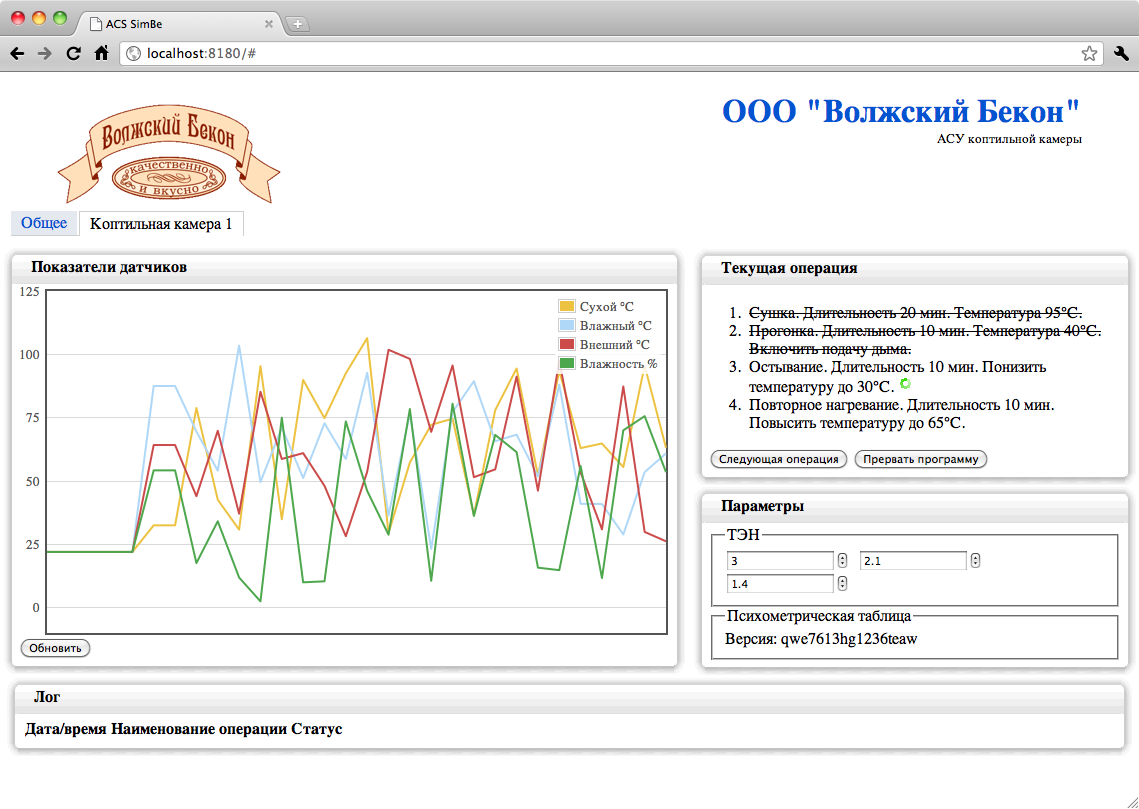
\includegraphics[bb=0 0 1200 800, clip, scale=0.4]{acs_if.png}}
	\caption{Интерфейс пользователя контролирующего сервиса}
	\label{img:acsIf}
\end{figure}

\subsubsection{Виды доступных операций}



\subsection{Разработка микропрограммы управляющего устройства}

% (http://www.complexdoc.ru/lib/ГОСТ%20Р%208.585-2001)
\subsubsection{Способ расчёта показателей датчиков температур по
ГОСТ Р 208.585-2001}
В качестве температурных датчиков устанавливаемых внутри объекта управления используются
термопары. Принцип получения показания температуры термопар основан на
термоэлектрическом эффекте Зеебека. Когда концы проводника находятся при разных температурах,
между ними возникает разность потенциалов, пропорциональная разности температур.
Коэффициент пропорциональности называют коэффициентом термоэдс.

Способ получения показаний температуры устройством управления универальной
ситемы терморегулирования осован на табличном методе поиска значения.
Основной его недостаток -- необходимость выделения 300 байт памяти микроконтроллера под
таблицу соответствия температуры и текущего показания термоэдс.
Однако он обладает следующими преимуществами:
\begin{itemize}
	\item{} сложность алгоритма вычисления значения температуры линецна и максимально занимает
		900 тактов;
	\item{} таблица соответствия может одновременно кодировать значение термоэдс с поправкой на
		ошибку считанного значения термоэдс, что необходимо выполнять ввиду нелинейной зависимости
		температуры и термоэдс, разброса чувствительности термопар составляющей 10-15\%, ошибки
		вносимой операционным усилителем, ошибки вносимой способом монтажа термопары на печатной плате;
	\item{} отсутствует необходимость использовать прецизионные сопротивления делителя
		напряжения операционного усилителя.
\end{itemize}

Для получения текущего значения температуры используется следующая формула:
\begin{equation}
	T_i = min_{tbl}(Adc(E_i \times{} K_{amp}) > x) 
\end{equation}
\begin{ESKDexplanation}
	\item[где ]{} $K_{amp}$ -- коэффициент усиления операционного уилителя,
	\item{} $E_i$ -- значение термоэдс,
	\item{} $T_i$ -- значение температуры,
	\item{} $Adc()$ -- функция преобразования аналогово сигнала в цифровой.
\end{ESKDexplanation}


Например для термопары типа Т, текущей температуры $1^oC$, $K_{amp}$ равным 100 и опорным напряжением
АЦП микроконтроллера 3.3 В получим:
$E_i = 0.000043$ В. Разрешение АЦП $= \frac{3.3}{2^{12}} = 0.000805$ В. Один градус температуры
кодируется $\frac{E_i \times{} K_{amp}}{\frac{3.3}{2^{12}}} = 5.34 $ значениями
беззнакового пребразования АЦП, а измеряемый диапазон температур составит от $0^oC$ до $862^oC$,
что в 4 раза превышает необходимую разрешающую способность.

\subsubsection{Методика расчёта компенсации холодного спая}
В местах подключения проводников термопары к управляющему устройству возникают дополнительные термоэдс.
В результате их действия на вход измерительной системы фактически поступает сумма сигналов от рабочей
термопары и от <<термопар>>, возникших в местах подключения.

Существуют различные способы избежать этого эффекта. Самым очевидным из них является поддержание
температуры холодного спая постоянной.

В управляющем устройстве используется техника <<компенсации холодного спая>>: температура холодного спая
измеряется датчиком температуры DS18B20, а затем величина термоэдс холодного спая программно
вычитается из сигнала термопары.

Места подключения термопары в управляющем устройстве расположены в непосредственной близости и имеют одинаковую
температуру, то есть находиться в изотермальной зоне. Датчик DS18B20 находиться в этой же зоне. Таким образом,
для компенсации холодного спая перед код чтения температуры с термопар производит чтение паказаний датчика DS18B20,
производит обратное табличное преобразование температуры в величену термоэдс градуированную по пораметрам
аналого-цифрового преобразователя и выполняет вычитание этих значений.

\subsubsection{Алгоритм управления силовой нагрузкой}

\subsubsection{Алгоритм сетевого взаимодействия управляющего устройства
с контолирующим сервером}
Для взаимодействия с контролирующим сервисом устройство управления использует сеть
стандарта Ethernet 802.3. Так как ни сам микроконтроллер at\-x\-mega\-128\-a3, ни микросхема
ecn28j60 не имеют большого буфера хранения входящих и исходящих сетевых пакетов,
было принято решение реализовать сетевое взаимодействие устройства с внешними устройствами
по упрощенной схеме итеративной обработки одного входного и одного выходного сетевого
пакета. Алгоритм сетевого взаимодейcтвия управляющего устройства с контролирующим сервисом представлен
на рисунке \ref{img:devProto}. Из представленного алгоритма видно, что все минимально необходимые
действия для осуществления работы по сети Ethernet 802.3, сосредоточены в одном конечном автомате.

\begin{figure}[h]
	\center{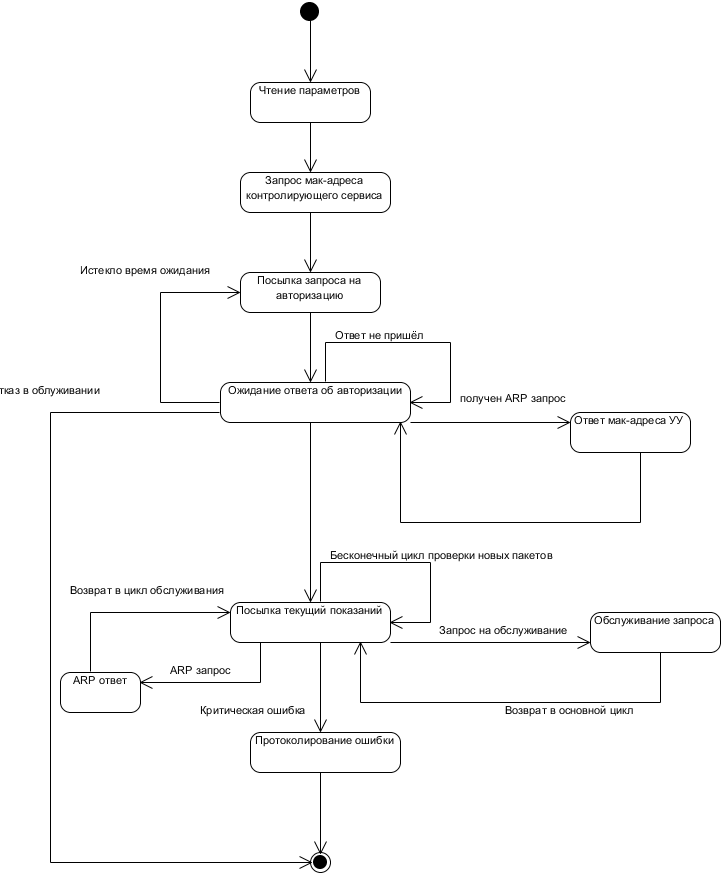
\includegraphics[bb=0 0 45 55, clip, scale=7.0]{dev_proto.png}}
	\caption{Протокол взаимодействия управляющего устройства и контроллирующего сервиса}
	\label{img:devProto}
\end{figure}

Представленный конечный автомат реализует ARP ''How has'' запрос, ARP ''How has'' ответ --
минимально необходимое подмножество функций протокола ARP для работы в сетях Ethernet 802.3.
В качестве транспортного протокола передачи данных было принято решение использовать
протокол UDP, всвязи с ограниченным количетвом оперативной памяти устройства управления, а так же
потому что алгоритм сетевого взаимодействия  предусматривает механизма повторения передачи
потерянных пакетов.

\subsubsection{Протокол взаимодействия управляющего устройства с контролирующим сервисом}

\subsubsection{Методика применения AES шифрования данных передаваемых
контроллирующему сервису}
Одна из порблем решаемых в порцессе разработки сетевого протокола 
взаимодействия управляющего устройства и контроллирующего сервиса
была проблема обеспечения безопасности передаваемых данных.


Конторллирующий сервис определяет, что принятые данные действительны
сравнивая пароль указаный в заголовке сетевого пакета. Однако,
при использования такого подхода, злоумышленник может прослушав
порходящий сетевой трафик получит этот пароль и использовать его
для формирования ложных запросов.


Для того, что бы избежать этого, заголовок пакета, содержащий пароль
и набор аппаратно специфичных данных, должен подвергаться дополнительному
кодированию с ипользованием секретного ключа, известного только
авторизованному устройству и контроллирующему сервису.


В качестве алгоритма кодирования данных заголовка пакета был использован
Advanced Encryption Standard. AES -- симметричный алгоритм блочного
шифрования, принятый в качестве стандарта шифрования правительством США
по результатам конкурса, организованного NIST в 1997 году, для замещения
алгоритма DES.


Причиной выбора именно этого алгоритма кодирования является
наличие аппаратной поддержки AES в микроконтроллерах XMega.


Благодаря наличию этого аппаратного модуля, порцедура кодирования
по алгоритму AES со стороны программного обеспечения микроконтроллера
сводиться к следующим шагам:
\begin{enumerate}
    \item{} Загрузить данные ключа в область памяти $AES.KEY$
        переферийного устройства AES кодирования.
    \item{} Загрузить шифруемые данные в область памяти $AES.STATE$.
    \item{} Установить параметры шифрования и флаг $AES_START_bm$ начала
        процедуры шифрования в конфигурационномй регистре $AES.CTRL$.
    \item{} Дождаться завршения шифрования, о чём сигнализирует
        флаги состояния в регистре состояния $AES.STATUS$.
    \item{} В рависимости от значения статуса, либо считать зашифрованные
        данные из области памяти $AES.STATE$, либо сообщить об ошибке
        шифрования.
\end{enumerate}


\subsubsection{Методика понижения потребляемого тока управляющим устройством
программным способом}

\subsubsection{Описание структуры классов микропрограммы управляющего устройства}

